\section{PNP Circuit}
Figure \ref{lab3_ex6_de} shows a very typical PNP transistor circuit.
Calculate $I_B$, $I_E$, and $I_C$ then simulate the circuit to double-check your calculation. Assume the current gain $\beta$ = 100.

\begin{figure}[H]
    \centering
    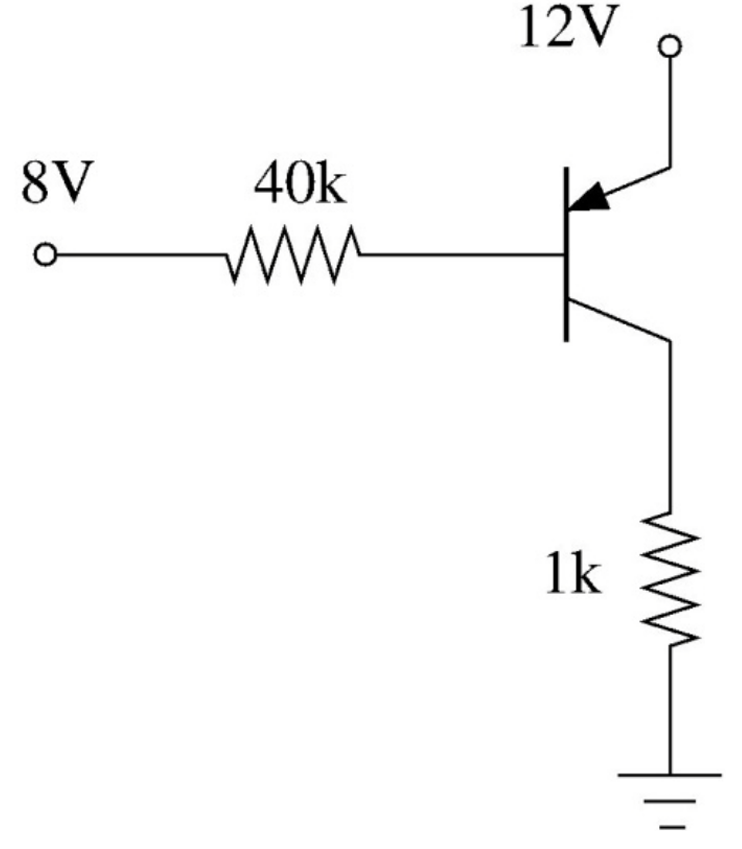
\includegraphics[width=0.5\linewidth]{graphics/ex6/f1.png}
    \caption{A PNP Circuit}
    \label{lab3_ex6_de}
\end{figure}

\subsection{Theoretical calculation}
\textit{\textbf{Notes:}}\\
\textit{Explanations, formulas, and equations are expected rather than only results.}

\begin{itemize}
    \item Vì đây là PNP transistor, nên $V_{EB}$ = 0.7 V (tránh nhầm lẫn với $V_{BE}$ trong NPN transistor).
    \item Áp dụng KVL: $$V_{EE} - V_{BB} - V_{EB} = I_B \times R_B $$
    $$ => I_B = \frac{V_{EE} - V_{BB} - V_{EB}}{R_B} = \frac{12V - 8V - 0.7V}{40k \Omega} = 82.5 \mu A $$
    \item $I_C = \beta \times I_B = 100 \times 82.5 \mu A = 8.25 mA $
    \item $I_E = I_B + I_C = 82.5\mu A + 8.25mA = 8.3325 mA$
\end{itemize}

\subsection{Simulation}
% \textbf{\textit{Your image goes here}}
\begin{figure}[H]
    \centering
    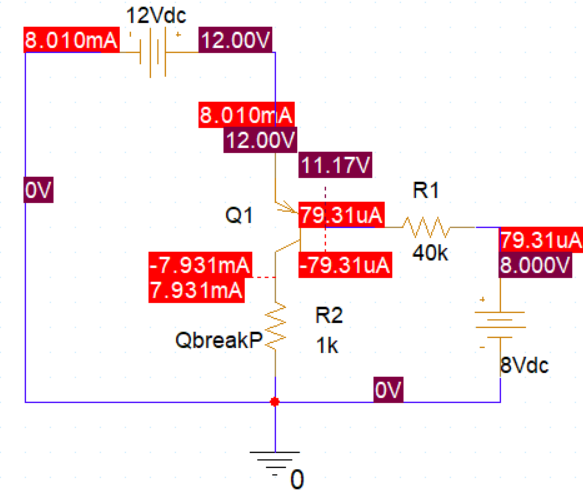
\includegraphics[width=0.9\linewidth]{graphics/ex6/f2.png}
    % \caption{A PNP Circuit}
\end{figure}

\subsection{Comparison}
$I_B$ (lý thuyết) = \dotfill$82.5 \mu A$ \dotfill $I_B$ (mô phỏng) =\dotfill $79.31 \mu A$\dotfill\bigskip\\
$I_C$ (lý thuyết) = \dotfill$ 8.250 mA$\dotfill $I_C$ (mô phỏng) = \dotfill $7.931mA$\dotfill\bigskip\\
$I_E$ (lý thuyết) = \dotfill$8.3325 mA$\dotfill $I_E$ (mô phỏng) = \dotfill$8.010mA $\dotfill\bigskip\\
